\documentclass[11pt]{article}
\usepackage[a4paper,margin=24mm]{geometry}
\usepackage[T1]{fontenc}
\usepackage[utf8]{inputenc}
\usepackage{lmodern,microtype,amsmath,amssymb,graphicx,booktabs,longtable}
\usepackage[numbers,sort&compress]{natbib}
\usepackage[colorlinks=true,allcolors=blue]{hyperref}
\usepackage{caption}
\usepackage[section]{placeins}
\captionsetup{font=small,labelfont=bf}
\setlength{\parskip}{4pt}\setlength{\parindent}{0pt}
\renewcommand{\thefigure}{S\arabic{figure}}
\renewcommand{\thetable}{S\arabic{table}}
\renewcommand{\thesection}{S\arabic{section}}
\title{Supporting Information\\[6pt]\large Local Chemical Environments Explain Charge-Definition Disagreement in Metal--Organic Frameworks}
\author{Hosein Alimardani, Shayan Abaei, and Mehrdad Asgari}
\date{}
\begin{document}
\maketitle\tableofcontents
\section{Data provenance, cohort, and fixed inputs}
The analysis uses QMOF Figshare article 13147324, version 18, archive file 59573735, with archive MD5 \nolinkurl{0d89aaf66f2c306e86e47fd91cb1346e}.\cite{Rosen2021,Rosen2022,QMOFv18} The available source population contains 20,372 structures and 2,312,743 atoms. The three-scheme finite-charge intersection contains 9,171 structures and 1,420,532 atoms. It includes 46,994 metal atoms in 9,165 structures. Cohort selection is availability based; the intersection is not claimed to be representative of every QMOF chemical class. Structures were not separately assembled from CoRE or CSD for this work, and charges were not recomputed with Gaussian or VASP.

The frozen configuration identifier is \nolinkurl{621045db53a892f1}. The source atom-order keys are QMOF identifier and atom index. Charge alignment checks include the element at each key and source site order. The full structural table and charge-target table remain separate from the compact plotting archive. The repository includes the descriptor manifest, graph decision, and numerical evidence reports. Release v1.0.0 separately deposits the full atom tables and completed production inputs; their file-level identities and retrieval instructions accompany the source.

\section{Graph construction and ambiguity}
Metals are classified by pymatgen's \nolinkurl{Element.is_metal}. Nonmetal pairs satisfy $0.40\leq d\leq 1.25(r_i+r_j)$, with all distances and ASE covalent radii in \AA.\cite{Ong2013,Larsen2017} Metal contact selection uses CrystalNN with \nolinkurl{weighted_cn=False}, \nolinkurl{cation_anion=False}, distance cutoffs $(0.5,1.0)$~\AA, \nolinkurl{x_diff_weight=0}, \nolinkurl{porous_adjustment=True}, \nolinkurl{search_cutoff=7.0}~\AA, and no fixed fingerprint length.\cite{Zimmermann2020} No oxidation states are assigned. CrystalNN's native no-oxidation-state radius fallback is retained; these radii are distinct from the ASE radii used for nonmetal cutoffs and normalized-distance features.

A metal center selects its metal--nonmetal contacts; ligand selection does not independently add or veto a contact. Either metal can select a metal--metal contact. Explicit reverse edges use the opposite lattice image. Identical site/image entries are deduplicated, while distinct periodic images are retained. First-shell descriptors summarize selected neighbors; two-hop descriptors count non-backtracking paths, including repeated destinations reached along distinct paths. A bond-distance spread is a distance statistic, not angular distortion or an electronic bond order.

The production table contains zero graph failures and 72 zero-neighbor atoms. Zero-neighbor sites are retained, since an isolated ion is not automatically an invalid structure. Diagnostic ambiguity flags include empty neighborhoods, metal--C/H contacts, selected metal--metal contacts, and a gap below 0.10 between the two largest CrystalNN coordination probabilities. The union flags 24,297 atoms, including 26.11\% of metal atoms. Flags are not adjudicated chemical bond-error labels. Radius sensitivity, extended contacts, and original-cutoff disagreement are separately recorded diagnostics.

The original connectivity comparison used 34 structures and 5,198 atoms. The accepted graph had 12,258 directed entries, no missing reverse edges, and four entries corresponding to additional legitimate images of indexed neighbors. Ten decisive calculations were replayed, and selected supercell checks reproduced mapped neighbor vectors and path counts for 1,132 sites. These checks establish the stated implementation properties; they do not establish universal chemical bond truth.

\section{Calibration, residual targets, and nested fits}
\subsection{Common charge mapping}
For each element, training-fold quantiles of $q^A$ define 12 bins. Weighted charge means supply an interpolated piecewise mapping, with endpoint-secant extrapolation. The common mapping predicts the ordered charge difference. It falls back to a training-fitted affine relation when there are fewer than 20 training structures, 100 atoms, or 20 distinct source-charge values. Affine slopes require variance above $10^{-6}\,e^2$ and 20 structures. Unobserved elements receive the training global offset. Calibration weights are inverse full structure size, renormalized within element. No held-out charges are used to fit bins, means, fallbacks, or residual models.

Let $c_{Z,k}(q^A)$ denote the common mapping trained outside fold $k$. All nested competitors predict
\begin{equation}
 \widehat\Delta_i=c_{Z_i,k}(q_i^A)+h_k(\mathbf{x}_i).
\end{equation}
The element residual mean is a recentering comparator. The flexible charge-only tree receives element identity/static central-element information and $q^A$. First-shell and then two-hop inputs are added to that same tree configuration. The target $q^B$, electronic bond orders, spin densities, and magnetic moments are excluded. No fitting statistic is embedded in the fixed structural dictionary. Native missing-value routing and histogram bins are learned from training atoms only.

\begin{figure}[!htbp]\centering
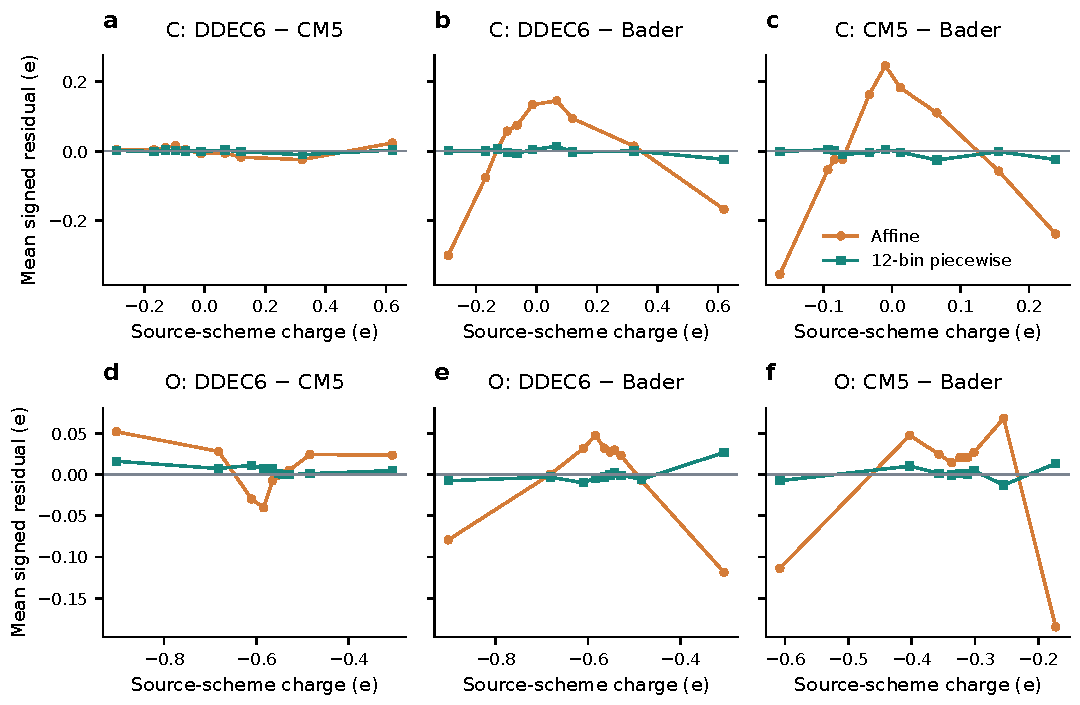
\includegraphics[width=\textwidth]{figures/Figure_S01_calibration.pdf}
\caption{Earlier affine and 12-bin piecewise charge-mapping diagnostics for carbon and oxygen in the original structure folds. Points are atom-weighted means in source-charge deciles of the pooled held-out atoms; bin counts and represented structures are saved in the plotting input. No uncertainty intervals are plotted. These illustrate calibration curvature before the stronger flexible charge-only residual control; they are not predictions of the final conditional structural model.}
\end{figure}

\subsection{Sampling and fixed tree settings}
For each fold, up to 12 atoms are retained per structure--element cell, with one reserved per available cell. A deterministic 160,000-atom cap is applied. Weights correct the retained sample to full-training atom proportions and inverse structure size. Every competitor uses the same keys and weights; evaluation includes all held-out atoms. Original-fold training keys are reused exactly. Blocked-fold samples are generated from the newly defined training structures only.

XGBoost settings are 100 estimators, maximum depth four, learning rate 0.08, minimum child weight 20, $L_2=5$, histogram construction with 128 bins, full row and column fractions, two threads, and random seed 20261109.\cite{Chen2016} No hyperparameter optimization or early stopping is performed. The existing charge-blind analyses remain distinct from this explicitly charge-conditioned follow-up. The comparison does not establish superiority over every possible model or scalar calibration.

\section{Validation groups, support, and statistical estimands}
The pinned metadata contain 5,408 nonempty MOFkey records, representing 5,114 distinct keys, and 8,468 distinct reduced formulas across the 9,171 structures. MOFkeys are source metadata, not identifiers reconstructed from names.\cite{Bucior2019} Connected components link equal nonempty exact MOFkeys or equal exact reduced formulas. There are 8,347 components; the largest contains 13 structures. The 1,414 nonsingleton records belong to 590 components. Under the original split, 1,189 records belonged to components spanning folds. Under the blocked split, no component crosses folds.

Components are sorted by decreasing size, with SHA256 hashing of the component identifier used to break ties; the exact seed prefix is recorded with the analysis source. Each is greedily assigned to the least populated fold, with fold-index tie breaking. Formula equality can block distinct structures and does not prove structural identity. MOFkey equality does not identify every broader family. No held-out-topology or unseen-element transfer result is claimed.

For atom weighting, absolute errors are pooled over atoms. For structure balancing, atom losses are first averaged within each structure and stated population, then averaged across represented structures. A component bootstrap resamples component sums of per-structure losses and the corresponding structure counts. Averaging component means equally would estimate a different quantity and is not used. Atom-weighted intervals analogously use component atom-error sums and atom counts. Paired increments use the same bootstrap draws for competing models, with 1,000 draws. The intervals are pointwise and conditional on the fitted models; they are not simultaneous discovery guarantees or uncertainty over every possible training run.

\begin{figure}[!htbp]\centering
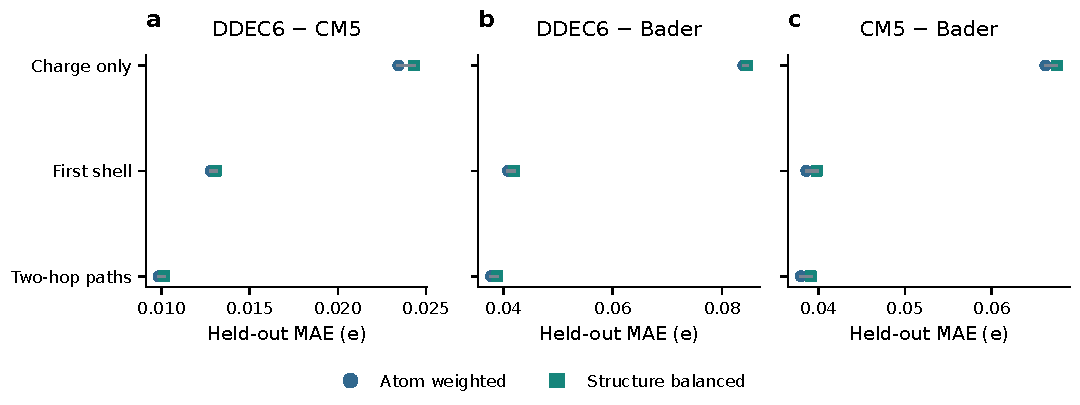
\includegraphics[width=\textwidth]{figures/Figure_S02_estimands.pdf}
\caption{Atom-weighted and structure-balanced MAE for the three nested conditional tree models under identifier/composition blocking. The two summaries weight the same 1,420,532 held-out atoms in 9,171 structures differently; points are estimates without plotted intervals. Comparisons should retain their declared population and weighting rather than mix the estimands.}
\end{figure}
\begin{figure}[!htbp]\centering
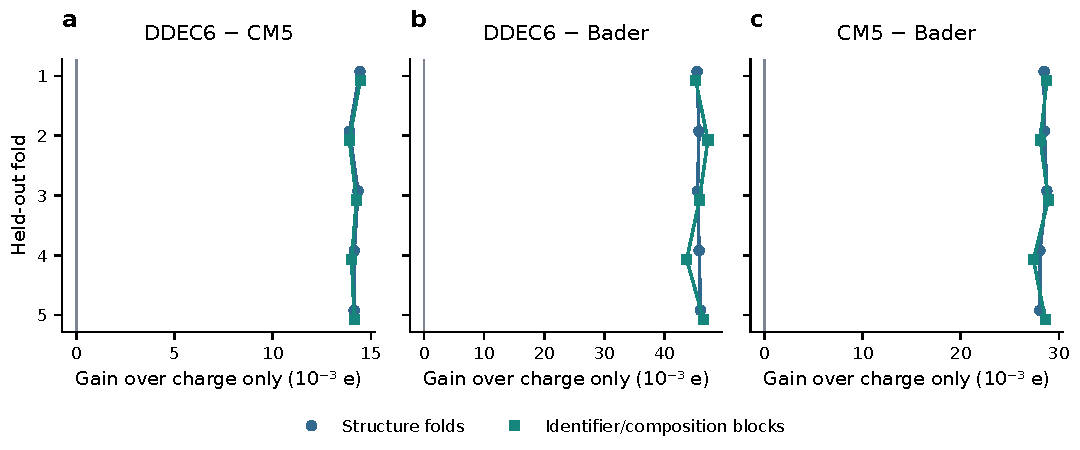
\includegraphics[width=\textwidth]{figures/Figure_S03_folds.pdf}
\caption{All-atom gain of the two-hop model over the flexible charge-only model in each of the five held-out folds, covering all 9,171 structures and 1,420,532 atoms. Positive gain is retained for each charge pair in both splitting schemes. Connecting lines organize fold-specific values and do not denote a temporal trajectory or an uncertainty interval.}
\end{figure}

\section{Environment definitions and atlas quantities}
Carbon classes are assigned with O-attachment taking priority, then N-attachment if O is absent, followed by strictly C/H-only neighbors. Monocoordinate H classes require one accepted neighbor of C, N, or O. O and N are classified by whether they have a selected metal neighbor. Metal donor classes are O-present/N-absent, N-present/O-absent, and mixed O/N; other donor elements can coexist. Unclassified and rare environments are retained in the full tables.

For the charge-only held-out residual $r_i=\Delta_i-\widehat\Delta_{i,\mathrm{charge}}$, the atlas separately reports raw signed difference, raw absolute difference, signed calibrated departure, absolute calibrated departure, and within-structure/environment residual standard deviation. An environment mean is first computed within each structure and then averaged over represented structures. The residual SD is likewise computed within each structure/environment and then averaged; it is not a pooled atom SD. A single-atom environment has SD zero by definition, not because its physical charge is known precisely.

For a paired contrast, the two environment means are subtracted within each structure containing both classes, and those differences are averaged. Contrast support differs from single-environment support. Main compact entries require at least 30 structures and 30 validation units. Counts, ambiguity fractions, lower-support entries, raw quantities, and graph coverage remain available in the complete numerical evidence. Pointwise contrast intervals are not multiplicity-adjusted; individual environment findings are descriptive associations rather than independent mechanistic discoveries.

\begin{figure}[!htbp]\centering
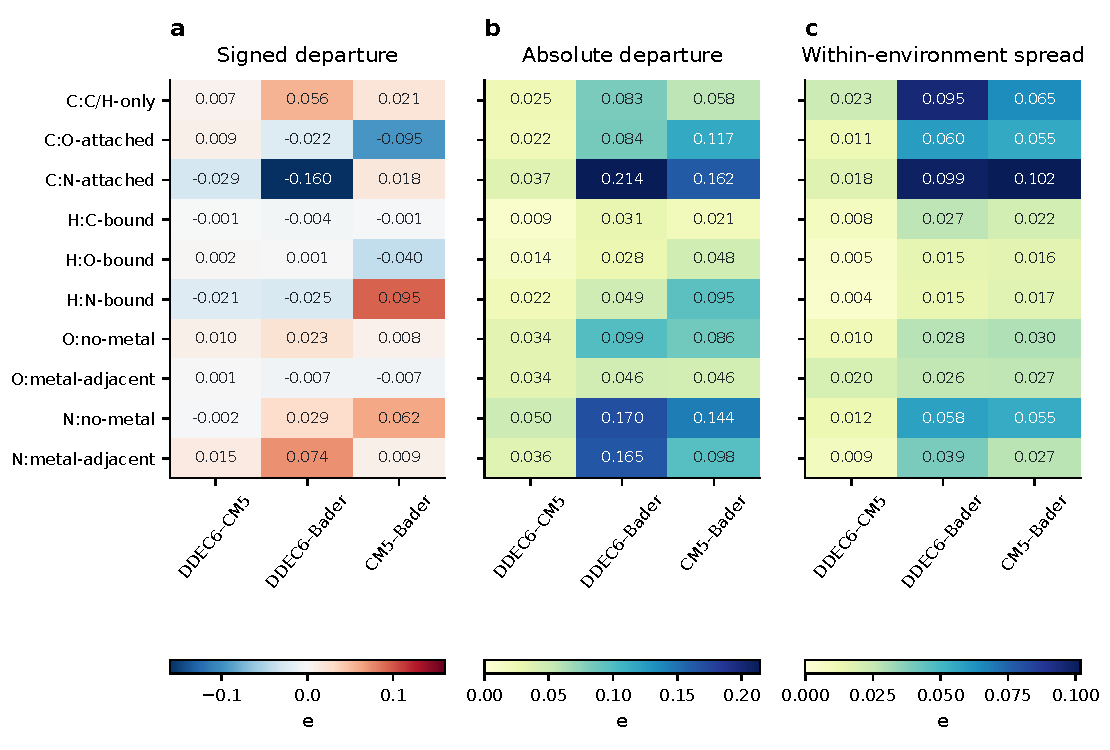
\includegraphics[width=\textwidth]{figures/Figure_S04_atlas.pdf}
\caption{Nonmetal environments after the flexible charge-only correction under identifier/composition blocking. Entries have at least 30 represented structures and 30 components; the represented population varies by environment. Signed departure, absolute departure, and within-structure/environment residual SD have separate color scales in e. Numbers are structure-balanced means without plotted uncertainty intervals. These descriptive quantities are neither charge-scheme accuracy scores nor calibrated physical uncertainty. Complete support and ambiguity columns are included in the accompanying CSV; no support filtering beyond the declared compact-atlas rule is introduced here.}
\end{figure}

\section{Finite graph sensitivity}
The 96-structure subset consists of 34 diagnostic structures and 62 deterministic identifier-hash selections. It contains 16,165 atoms and is fixed independently of the closeout outcomes. Nonmetal cutoffs 1.20 and 1.30 are compared with the accepted 1.25 while all accepted metal-involving indexed-site/image edges remain fixed. First-shell and two-hop features and environment labels are recomputed, but charge-only residuals are held fixed. Both available-pair and common-pair results are saved; Figure~\ref{fig:si-cutoff} uses the common paired-structure intersection.

The 1.20 setting changes no first shells. The wider 1.30 cutoff adds 12 unoriented image-aware contacts, changes 18 first-shell and 38 two-hop feature records, and changes none of the tested headline environment assignments. Common-pair effects are numerically unchanged. Some contrasts have small paired support in this subset; the result must not be generalized to the full chemical space. Six H sites have near-midpoint O--H--O geometries, exposing an ambiguity not settled by stable headline contrasts.

\begin{table}[!htbp]
\centering\small
\caption{Central-metal MAE and paired two-hop gain under identifier/composition blocking, in e. The global models are evaluated on 46,994 metal atoms in 9,165 structures. Pointwise 95\% component-bootstrap intervals condition on the fitted models.}
\label{tab:si-metal}
\setlength{\tabcolsep}{3pt}
\begin{tabular}{lrrrrl}
\toprule
Charge pair & Charge only & First shell & Two-hop & Gain & 95\% interval \\
\midrule
DDEC6--CM5 & 0.02694 & 0.02189 & 0.02202 & 0.00493 & [0.00451, 0.00533] \\
DDEC6--Bader & 0.02044 & 0.02241 & 0.02851 & -0.00807 & [-0.00857, -0.00749] \\
CM5--Bader & 0.02959 & 0.02962 & 0.02868 & 0.00091 & [0.00049, 0.00137] \\
\bottomrule
\end{tabular}
\end{table}


The earlier metal graph diagnostic applies alternative graphs to fixed, earlier metal-only fits. The plotted taper shift is $+0.10$~\AA\ at both CrystalNN taper endpoints; the other stress graph uses the original radius-cutoff rule. These predictions evaluate 508 metal atoms across the subset's 96 structures. They are a separate follow-up, not a newly fitted conditional metal ladder. No whole-cohort alternative-graph retraining is claimed.

\begin{figure}[!htbp]\centering
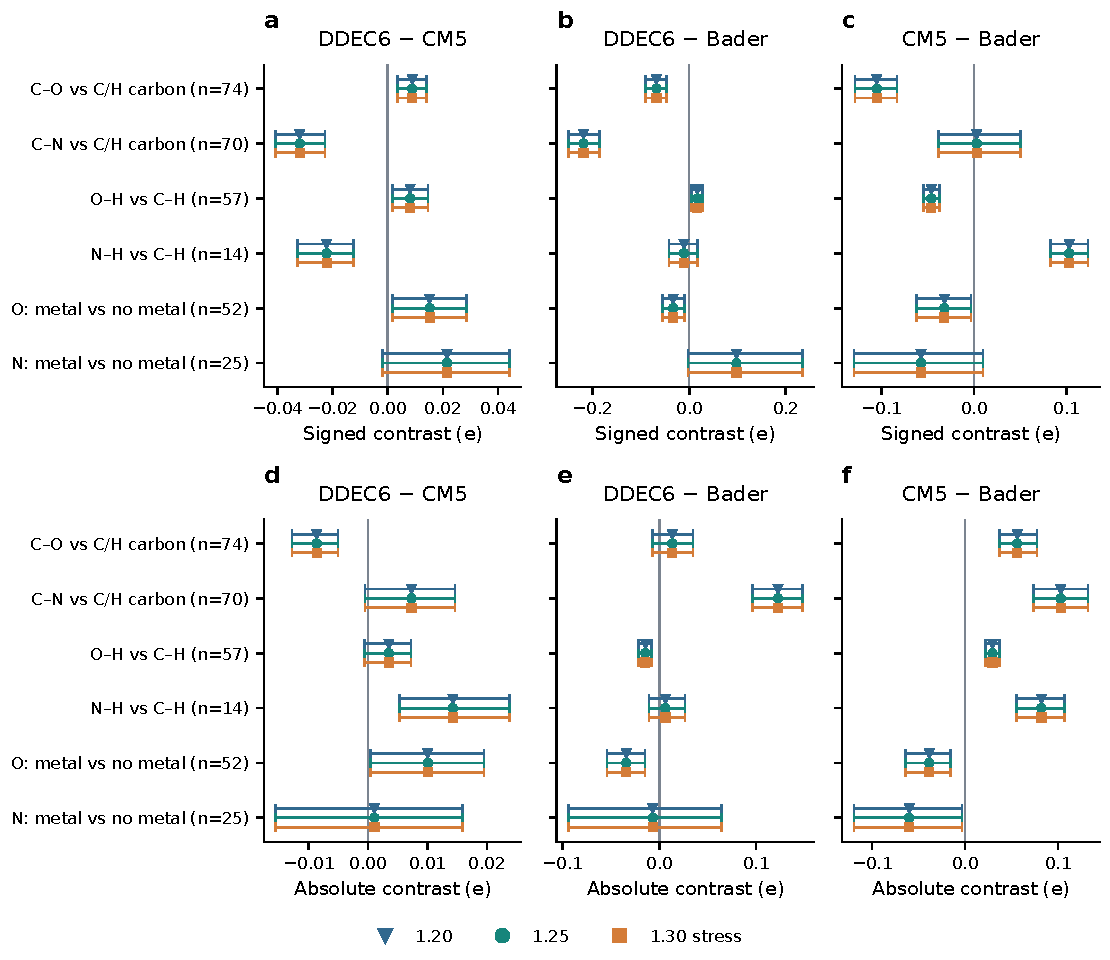
\includegraphics[width=\textwidth]{figures/Figure_S05_cutoff_contrasts.pdf}
\caption{Signed and absolute calibrated-departure contrasts on common paired structures in the fixed graph subset. Three nonmetal cutoff scales are shown at vertically offset positions; effects and intervals coincide where assignments are unchanged. Original-fold flexible charge-only residuals and accepted metal edges are held fixed. Error bars are saved pointwise 95\% structure-bootstrap intervals. Small paired populations limit some contrast-specific conclusions.}\label{fig:si-cutoff}
\end{figure}

\section{Reproduction scope and source inventory}
The figure pipeline reads only frozen CSV estimates and exports PDF, editable SVG, and 400-dpi PNG files. It neither refits models nor recomputes uncertainty intervals. The \nolinkurl{PROVENANCE.json} file maps each plotting input to its source and SHA256 digest. The accompanying analysis source is preserved separately from the new figure source. Compact numerical reconciliation, full model refitting, and source-to-descriptor reproduction are distinct operations.

Release \href{https://github.com/alimardani76/chamm/releases/tag/v1.0.0}{v1.0.0} at \url{https://github.com/alimardani76/chamm} separates three reproduction levels. Figure reproduction uses only compact plotting inputs. Compact numerical reconstruction reaggregates per-structure losses, environment summaries, and contrast vectors, checking principal paired bootstrap intervals and split/training separation. Both levels are verified from a clean checkout. Full model/descriptor reproduction additionally uses the deposited frozen structural-feature and charge-target tables, original and blocked training samples, pinned QMOF archive, metadata, accepted caches, and 96-structure manifest. A retrieval script verifies the deposit SHA256 and extracted file hashes. The reusable numeric feature matrix is regenerated from the supplied frozen table. The release verifies input integrity and representative descriptor/model replay, but does not claim a fresh end-to-end refit of all models or a whole-cohort descriptor rebuild. Original observed dependency records and the independently tested release environment are provided separately.

The analysis characterizes relationships between existing charge definitions; none is a reference truth. The exploratory metal-only result is disclosed alongside the final global conditional metal failure. The archived numerical evidence retains positive, negative, low-support, and ambiguous cases so that the reported scope can be assessed directly.
\clearpage
\bibliographystyle{unsrtnat}\bibliography{references}
\end{document}
